         \chapter{The particles that substances are made of}\fancyfoot[LO,RE]{Chemistry: Matter and materials}
\label{chap:composition}
    \setcounter{figure}{1}
    \setcounter{subfigure}{1}
    \label{m38120}
\section{Atoms and compounds}
\subsection*{The atom as the building block of matter}
            \nopagebreak
%\label{m38120*cid2} $ \hspace{-5pt}\begin{array}{cccccccccccc}   \end{array} $ \hspace{2 pt}\raisebox{-0.2em}{
\includegraphics[height=1em]{../icons/www.pdf}} {(section shortcode: P10053 )} \par 
\label{m38120*id307092}We have seen that different materials have different properties. But what would we find if we were to break down a material into the parts that make it up (i.e. it's microscopic structure)? And how is it that this microscopic structure is able to give matter all its different properties?\par 
\chapterstartvideo{VPaxx}
\begin{minipage}{.6\textwidth}
\label{m38120*id307099}The answer lies in the smallest building block of  matter: the \textbf{atom}. It is the \textsl{type} of atoms, and the way in which they are \textsl{arranged} in a material, that affects the properties of that substance. This is similar to building materials. We can use bricks, steel, cement, wood, straw (thatch), mud and many other things to build structures from. The choice of atoms affects the properties of matter in the same way as the choice of building material affects the properties of the structure, \par 
\end{minipage}
\begin{minipage}{.4\textwidth}
 \begin{center}
\includegraphics[width=0.6\textwidth]{photos/atom_model_kit.jpg}
 \end{center}
\end{minipage}

 \label{m38120*id307459}It is not often that substances are found in atomic form (just as you seldom find a building or structure made from one building material). Normally, atoms are bonded (joined) to other atoms to form \textbf{compounds} or \textbf{molecules}. It is only in the \textsl{noble gases} (e.g. helium, neon and argon) that atoms are found individually and are not bonded to other atoms. We looked at some of the  reasons for this in earlier chapters.
    \subsection*{Compounds}
            \nopagebreak
%            \label{m38120*cid3} $ \hspace{-5pt}\begin{array}{cccccccccccc}   \end{array} $ \hspace{2 pt}\raisebox{-0.2em}{
\includegraphics[height=1em]{../icons/www.pdf}} {(section shortcode: P10054 )} \par 

            \label{m38120*fhsst!!!underscore!!!id74}
\Definition{ Compound} {  A compound is a group of two or more different atoms that are attracted to each other by relatively strong forces or bonds. The atoms are combined in definite proportions.   } 
Compounds can be divided into \textbf{molecular compounds} (molecules), \textbf{ionic compounds} (salts) and \textbf{metallic compounds} (metals).
\begin{itemize}[noitemsep]
 \item \textbf{Molecular compounds} form as a result of covalent bonding where electrons are shared between non-metal atoms.
\item \textbf{Ionic compounds} form as a result of ionic bonding where electrons are transferred from metals to non-metals. 
\item \textbf{Metals} are formed as a result of metallic bonding where metal atoms lose their outer electrons to form a lattice of regularly spaced positive ions and a 'pool' of delocalised electrons that surround the positive ions. 
\end{itemize}
The following diagram illustrates how compounds can be subdivided by the type of bonding and the structure.
\begin{figure}[H]
 \begin{center}
  \begin{pspicture}(-6,0.5)(6,5)
%\psgrid[gridcolor=lightgray]
\rput(0,4.8){\textbf{COMPOUNDS}}
\psline(-3,4)(-3,4.4)(4.5,4.4)(4.5,4)
\rput(-3,3.8){\textbf{Covalent molecular structures}}
\rput(4.8,3.8){\textbf{Network structures}}
\psline(4.5,3)(4.5,3.6)
\psline(7.5,3)(7.5,3.4)(1.5,3.4)(1.5,3)
%covalent molecular
\rput(-3,3.3){water ($\text{H}_{2}\text{O}$)}
\rput(-3,2.8){oxygen ($\text{O}_{2}$)}
\rput(-3,2.3){sulphur ($\text{S}_{8}$)}
\rput(-3,1.8){buckyballs ($\text{C}_{60}$)}
%putting other text
\rput(4.5,2.8){\textbf{ionic network}}
\rput(4.5,2.4){\textbf{structures}}
\rput(1.2,2.8){\textbf{covalent network}}
\rput(1.2,2.4){\textbf{structures}}
\rput(7.8,2.8){\textbf{metallic network}}
\rput(7.8,2.4){\textbf{structures}}
%ionic structures
\rput(4.5,1.9){sodium chloride ($\text{NaCl}$)}
\rput(4.5,1.4){barium sulphate ($\text{BaSO}_{4}$)}
\rput(4.5,0.9){silver iodide ($\text{AgI}$)}
%metallic structures
\rput(7.8,1.9){copper ($\text{Cu}$)}
\rput(7.8,1.4){iron ($\text{Fe}$)}
\rput(7.8,0.9){gold ($\text{Au}$)}
%other covalent
\rput(1.2,1.9){diamond ($\text{C}$)}
\rput(1.2,1.4){graphite ($\text{C}$)}
\rput(1.2,0.9){silica ($\text{SiO}_{2}$)}
\end{pspicture}
 \end{center}
\end{figure}
\subsubsection*{Covalent molecular structures}
Relatively small molecules are called \textbf{covalent molecular structures}. These exist and interact as separate molecules. Oxygen ($\text{O}_{2}$), water ($\text{H}_{2}\text{O}$), octane ($\text{C}_{8}\text{H}_{18}$), sulphur ($\text{S}_{8}$) and buckminsterfullerene ($\text{C}_{60}$, buckyballs) are all examples of covalent molecular structures. \\
\begin{figure}[H]
  \begin{center}
  \begin{minipage}[c]{5 cm}
    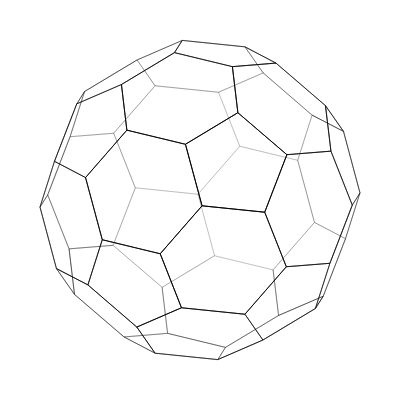
\includegraphics[width=0.6\textwidth]{photos/Buckyball_Carbon.png} \\
    \textsl{buckminsterfullerene}
  \end{minipage}
  \begin{minipage}[c]{5 cm}
    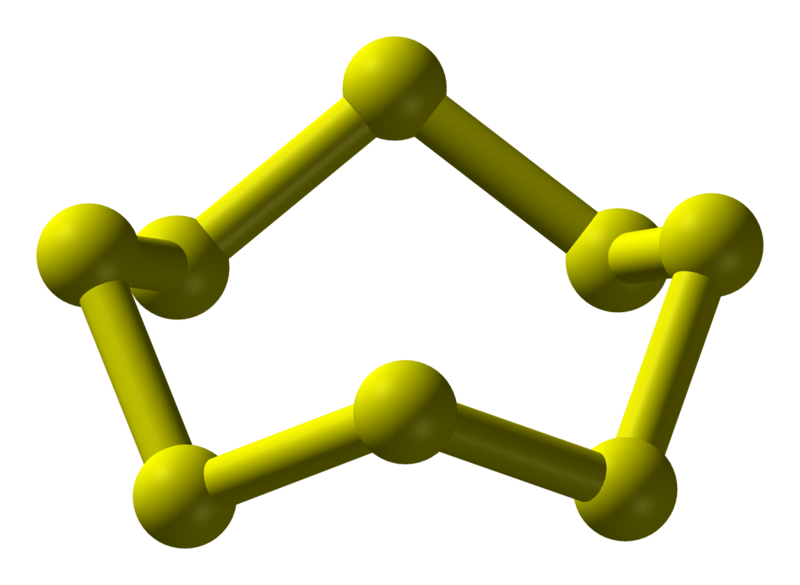
\includegraphics[width=0.6\textwidth]{photos/sulphur_wikipedia.png}  \\ 
    \textsl{sulphur}
  \end{minipage}
\caption{Examples of covalent molecular structures}
\end{center}
\end{figure}

\subsubsection*{Network structures}
Compounds that exist as giant repeating lattice structures are called network structures. Examples include \textbf{covalent molecules} such as diamond, graphite and silica. \textbf{Ionic substances} are also network structures, for example a sodium chloride crystal is a huge lattice of repeating units made of sodium and chloride ions. All substances formed as a result of ionic bonding are network structures. \textbf{Metals} exist as large continuous lattice structures and are also classified as network structures. For example copper, zinc and iron can be seen as a giant crystals and are therefore considered to be network structures.
\mindsetvid{Animation of diamond and graphite}{VPazc}
\begin{figure}[H]
  \begin{center}
  \begin{minipage}[c]{4.5 cm}
    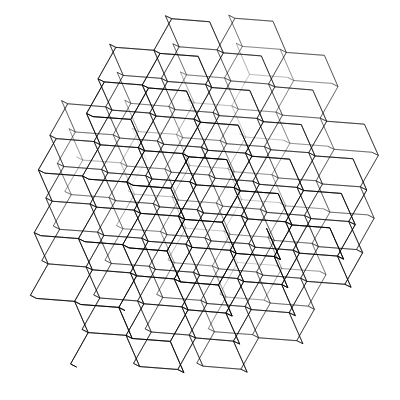
\includegraphics[width=0.8\textwidth]{photos/Diamond_Carbon.png} \\
    \textsl{covalent network}
  \end{minipage}
  \begin{minipage}[c]{4.5 cm}
    \includegraphics[width=0.8\textwidth]{photos/BaSO4_wikipedia.png}  \\ 
    \textsl{ionic network}
  \end{minipage}
  \begin{minipage}[c]{4.5 cm}
    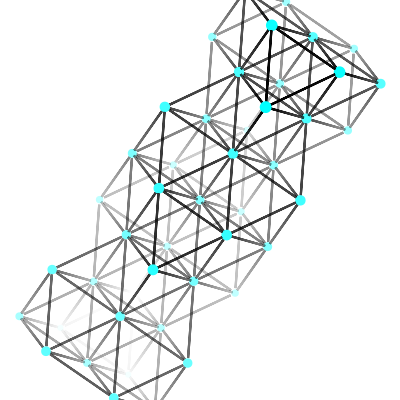
\includegraphics[width=0.8\textwidth]{photos/copper_structure.png}   \\ 
    \textsl{metallic network}
  \end{minipage}
\caption{Examples of network structures}
\end{center}
\end{figure}

\subsection*{Representing molecules}
            \nopagebreak
\label{m38120*id307557}The structure of a molecule can be shown in many different ways. Sometimes it is easiest to show what a molecule looks like by using different types of \textbf{diagrams}, but at other times, we may decide to simply represent a molecule using its \textbf{chemical formula} or its written name. 

\subsubsection*{Using formulae to show the structure of a molecule}
A \textbf{chemical formula} is an abbreviated (shortened) way of describing a compound. In chapter~\ref{chap:classification}, we saw how chemical compounds can be represented using element symbols from the periodic table. A chemical formula can also tell us the \textsl{number} of atoms of each element that are in a compound and their \textsl{ratio} in that compound. If the compound is a covalent molecular compound then we can use the molecular formula.

 \Definition{Molecular formula} {The molecular formula is a concise way of expressing information about the atoms that make up a particular covalent molecular compound. The molecular formula gives the exact number of each type of atom in the molecule. } 

For example in figure~\ref{fig:representing isobutane} the molecular formula of 2-methyl propane is $\text{C}_{4}\text{H}_{10}$. This tells us that there are $4$ carbon atoms and $10$ hydrogen atoms in this molecule, i.e the ratio of carbon to hydrogen is $4:10$. But we can simplify this ratio to: $2:5$. This gives us the \textbf{empirical formula} of the molecule. 

\Definition{  Empirical formula } { \label{m38120*meaningfhsst!!!underscore!!!id93}
The empirical formula is a way of expressing the \textsl{relative} number of each type of atom in a chemical compound. The empirical formula does not show the exact number of atoms, but rather the simplest \textsl{ratio} of the atoms in the compound. }

\Note{The empirical and the molecular formulae can be the same. For example in carbon dioxide the molecular formula is $\text{CO}_{2}$. This is also the empirical formula since it is the simplest ratio. }

The empirical formula is useful when we want to write the formula for \textsl{network structures}. Since network structures may consist of millions of atoms, it is impossible to say exactly how many atoms are in each unit. It makes sense then to represent these units using their empirical formula. So, in the case of a metal such as copper, we would simply write $\text{Cu}$, or if we were to represent a unit of sodium chloride, we would simply write $\text{NaCl}$. Chemical formulae (i.e. the molecular or the empirical formula) therefore tell us something about the \textsl{types} of atoms that are in a compound and the \textsl{ratio} in which these atoms occur in the compound, but they don't give us any idea of what the compound actually looks like, in other words its \textsl{shape}. To show the shape of compounds we have to use diagrams. The simplest type of diagram that can be used to describe a compound is its \textbf{structural formula}. The structural formula for 2-methyl propane is shown in figure~\ref{fig:representing isobutane}. 
   \setcounter{subfigure}{0}
\begin{figure}[H]
\begin{center}
\begin{pspicture}(-5,-1)(5,0.6)
%\psgrid[gridcolor=lightgray]
\rput(-3,0){(a) \textbf{C$_{4}$H$_{10}$}}
\rput(-1,0){(b) \textbf{C$_{2}$H$_{5}$}}
\rput(0.5,0){(c)}
% \rput(2,0){\chemfig{CH(-[2]CH_3)(-[7]CH_3)(-[5]CH_3)}}
\rput(2,0){
\rput(0.65,1.65){\large $\text{CH}_3$}
\rput(0.1,0){\large $\text{CH}_3$}
\rput(1.2,0){\large $\text{CH}_3$}
\rput(0.55,0.9){\large $\text{CH}$}
\psline[linewidth=0.04cm](0.5,1.05)(0.5,1.5)
\psline[linewidth=0.04cm](0,0.2)(0.4,0.7)
\psline[linewidth=0.04cm](1,0.2)(0.6,0.7)}
\end{pspicture}
\caption{Diagram showing (a) the chemical, (b) the empirical and (c) the structural formula of 2-methyl propane}
\label{fig:representing isobutane}
\end{center}
\end{figure} 

% \subsubsection*{Using formulae to show the structure of a molecule.}
% A \textbf{chemical formula} is an abbreviated (shortened) way of describing a molecule, or some other chemical substance. In chapter~\ref{chap:classification}, we saw how chemical compounds can be represented using element symbols from the Periodic Table. A chemical formula can also tell us the \textsl{number} of atoms of each element that are in a molecule and their \textsl{ratio} in that molecule. For example, the chemical formula for a molecule of carbon dioxide is ${\text{CO}}_{2}$. This formula is called the \textbf{molecular formula} of that compound. The formula tells us that in one molecule of carbon dioxide, there is one atom of carbon and two atoms of oxygen. The ratio of carbon atoms to oxygen atoms is 1:2.\par
%         \label{m38120*fhsst!!!underscore!!!id87}
%  \Definition{Molecular formula} { \label{m38120*meaningfhsst!!!underscore!!!id87}
% The molecular formula is a concise way of expressing information about the atoms that make up a particular chemical compound. The molecular formula gives the exact number of each type of atom in the molecule. } 
% 
% A molecule of glucose has the molecular formula: ${\text{C}}_{6}{\text{H}}_{12}{\text{O}}_{6}$. In each glucose molecule, there are six carbon atoms, twelve hydrogen atoms and six oxygen atoms. The ratio of carbon:hydrogen:oxygen is 6:12:6. We can simplify this ratio to write 1:2:1 (this means that for every one carbon atom there must be two hydrogen atoms and one oxygen atom), or if we were to use the element symbols, the formula would be written as ${\text{CH}}_{2}\text{O}$. This is called the \textbf{empirical formula} of the molecule.\\
%         \label{m38120*fhsst!!!underscore!!!id93}
% \Definition{   \label{id2456770}\textbf{ Empirical formula }} { \label{m38120*meaningfhsst!!!underscore!!!id93}
% The empirical formula is a way of expressing the \textsl{relative} number of each type of atom in a chemical compound. In most cases, the empirical  formula does not show the exact number of atoms, but rather the simplest \textsl{ratio} of the atoms in the compound.  } 

% The empirical formula is useful when we want to write the formula for \textsl{network structures}. Since network structures may consist of millions of atoms, it is impossible to say exactly how many atoms are in each unit. It makes sense then to represent these units using their empirical formula. So, in the case of a metal such as copper, we would simply write $\text{Cu}$, or if we were to represent a molecule of sodium chloride, we would simply write $\text{NaCl}$. Chemical formulae therefore tell us something about the \textsl{types} of atoms that are in a compound and the \textsl{ratio} in which these atoms occur in the compound, but they don't give us any idea of what the molecule actually looks like, in other words its \textsl{shape}. To show the shape of compounds we can use diagrams. Another type of formula that can be used to describe a compound is its \textbf{structural formula}. A structural formula uses a graphical representation to show a compound's structure                    
% (Figure \ref{fig:representing isobutane}).
%     \setcounter{subfigure}{0}
% \begin{figure}[h]
% \begin{center}
% \begin{pspicture}(-5,-1)(5,0.6)
% %\psgrid[gridcolor=lightgray]
% \rput(-3,0){(a) \textbf{C$_{4}$H$_{10}$}}
% \rput(-1,0){(b) \textbf{C$_{2}$H$_{5}$}}
% \rput(0.5,0){(c)}
% \rput(2,0){\chemfig{CH(-[2]CH_3)(-[7]CH_3)(-[5]CH_3)}}
% \end{pspicture}
% \caption{Diagram showing (a) the molecular, (b) the empirical and (c) the structural formula of 2-methylpropanone}
% \label{fig:representing isobutane}
% \end{center}
% \end{figure}      
\label{m38120*uid4}\subsubsection*{Using diagrams to show the structure of a compound}
Diagrams of compounds are very useful because they help us to picture how the atoms are arranged in the compound and they help us to see the shape of the compound. There are three types of diagrams that are commonly used:
\label{m38120*id307860}\begin{itemize}[noitemsep]
\item \textbf{Wireframe or stick models} \\
In this model, the bonds between atoms are shown as 'sticks'. These 'sticks' are coloured to show which atoms are bonding.
\item \textbf{Ball and stick models} \\
This is a 3-dimensional molecular model that uses 'balls' to represent atoms and 'sticks' to represent the bonds between them. The centres of the atoms (the balls) are connected by straight lines which represent the bonds between them.
\item \textbf{Space-filling models} \\
This is also a 3-dimensional molecular model. The atoms are represented by spheres.
\end{itemize}
Table~\ref{tab:atommodels} shows examples of the different types of models for all the types of compounds.
\begin{table}[H]
 \begin{center}
  \begin{tabular}{|p{2cm}|l|l|l|l|}  \hline
   & \textbf{Covalent molecular} & \textbf{Covalent network} & \textbf{Ionic network} & \textbf{Metallic network}   \\ \hline
\textbf{Name of compound} & glucose & graphite & silver chloride & zinc \\ \hline
\textbf{Formula} & $\text{C}_{6}\text{H}_{12}\text{O}_6$ or $\text{C}\text{H}_{2}\text{O}$ & $\text{C}$ & $\text{AgCl}$ & $\text{Zn}$  \\ \hline
\textbf{Stick model} & 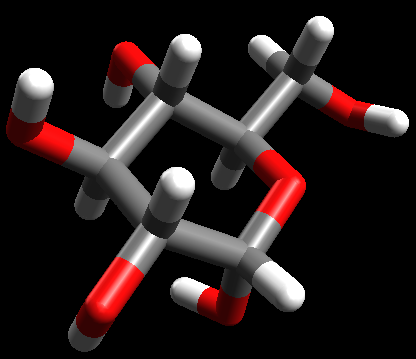
\includegraphics[width=.2\textwidth]{photos/glucose_wire.png} & \includegraphics[width=.2\textwidth]{photos/graphite.png} & \scalebox{0.5} % Change this value to rescale the drawing.
{
\begin{pspicture}(0,-1.78)(2.02,1.78)
  \psset{Alpha=75,Beta=20}
  \psset{xMin=-3,xMax=3,yMin=-3,yMax=3,zMin=-3,zMax=3}
%   \pstThreeDCoor
   \pstThreeDLine(-2,-2,-2)(-2,-2,2) \pstThreeDLine(-2,-2,2)(-2,2,2)
   \pstThreeDLine(-2,2,2)(-2,2,-2) \pstThreeDLine(-2,2,-2)(-2,-2,-2)
   \pstThreeDLine(-2,-2,0)(-2,2,0) \pstThreeDLine(-2,0,-2)(-2,0,2)

   \pstThreeDLine(0,-2,-2)(0,-2,2) \pstThreeDLine(0,-2,2)(0,2,2)
   \pstThreeDLine(0,2,2)(0,2,-2) \pstThreeDLine(0,2,-2)(0,-2,-2)
   \pstThreeDLine(0,-2,0)(0,2,0) \pstThreeDLine(0,0,-2)(0,0,2)

  \pstThreeDLine(2,-2,-2)(2,-2,2) \pstThreeDLine(2,-2,2)(2,2,2)
  \pstThreeDLine(2,2,2)(2,2,-2) \pstThreeDLine(2,2,-2)(2,-2,-2)
  \pstThreeDLine(2,-2,0)(2,2,0) \pstThreeDLine(2,0,-2)(2,0,2)

  \pstThreeDLine(-2,2,2)(2,2,2) \pstThreeDLine(-2,0,2)(2,0,2)
  \pstThreeDLine(-2,-2,2)(2,-2,2)
  \pstThreeDLine(-2,2,0)(2,2,0) \pstThreeDLine(-2,0,0)(2,0,0)
  \pstThreeDLine(-2,-2,0)(2,-2,0)
  \pstThreeDLine(-2,2,-2)(2,2,-2) \pstThreeDLine(-2,0,-2)(2,0,-2)
  \pstThreeDLine(-2,-2,-2)(2,-2,-2)
\end{pspicture} 
}  & \includegraphics[width=.15\textwidth]{photos/zinc_sticks.png} \\ \hline
\textbf{Ball-and-stick model} & \includegraphics[width=.2\textwidth]{photos/glucose_balls.png}  & 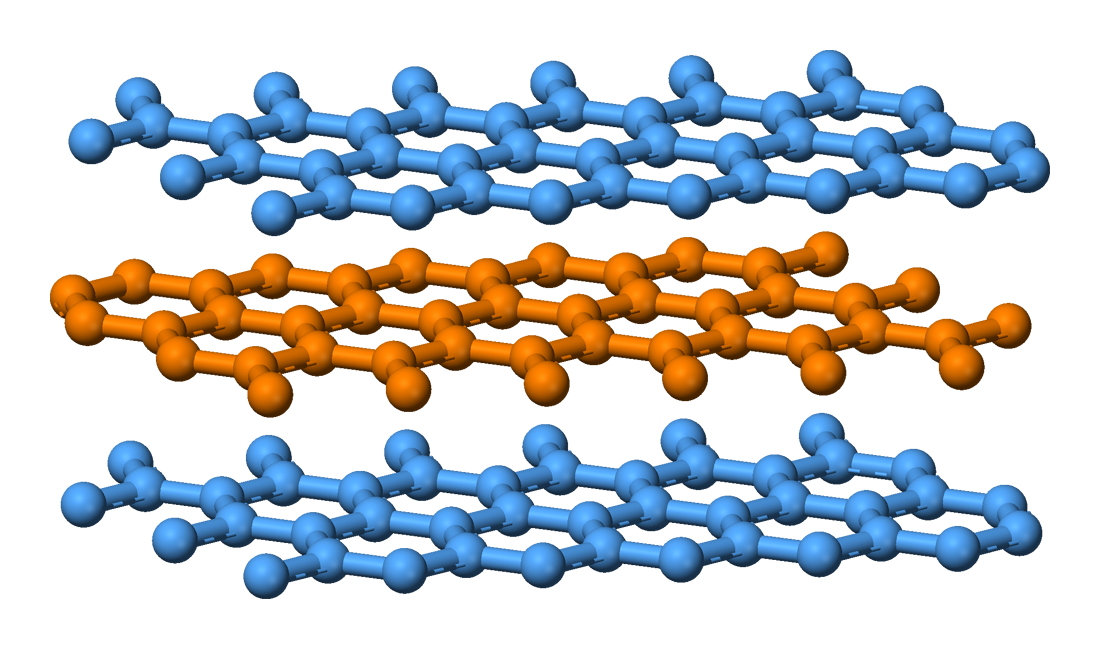
\includegraphics[width=.2\textwidth]{photos/graphite_wikipedia.png} & 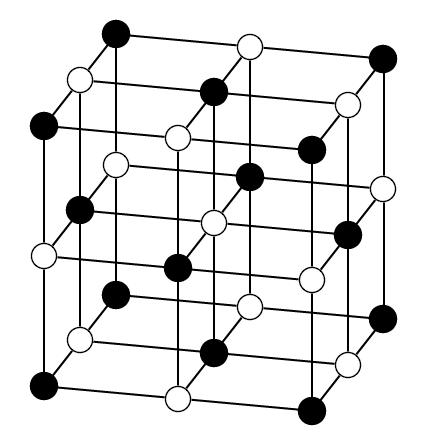
\includegraphics[width=.2\textwidth]{photos/silver_chloride_ballstick.png} & \includegraphics[width=.1\textwidth]{photos/zinc_ball_stick.png} \\ \hline
\textbf{Space-filling model} & \includegraphics[width=.1\textwidth]{photos/glucose_spacefill.png}  & 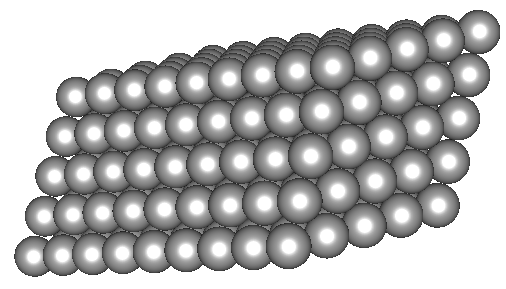
\includegraphics[width=.2\textwidth]{photos/graphite_spacefill.png} & \includegraphics[width=.1\textwidth]{photos/silverchloride_spacefill_wikipedia.png} & 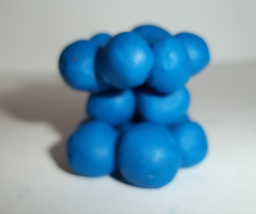
\includegraphics[width=.1\textwidth]{photos/zinc_spacefill.png} \\ \hline
  \end{tabular}
 \end{center}
\caption{Different representations for compounds}
\label{tab:atommodels}
\end{table}
\pagebreak
\begin{activity}{Representing compounds}
A list of substances is given below. Make use of atomic model kits, play dough and toothpicks, or coloured polystyrene balls and skewer sticks to represent each of the substances in three dimensional structures.\\
\begin{minipage}{.4\textwidth}
\begin{itemize}[noitemsep]
 \item glucose ($\text{C}_{6}\text{H}_{12}\text{O}_{6}$)
\item silica ($\text{SiO}_{2}$)
\item sodium chloride ($\text{NaCl}$)
\item sulphur ($\text{S}_{8}$)
\item diamond ($\text{C}$)
\item graphite ($\text{C}$)
\item buckyballs( $\text{C}_{60}$)
\item sucrose ($\text{C}_{12}\text{H}_{22}\text{O}_{11}$)
\item copper ($\text{Cu}$)
\end{itemize}
\end{minipage}
\begin{minipage}{.6\textwidth}
\begin{center}
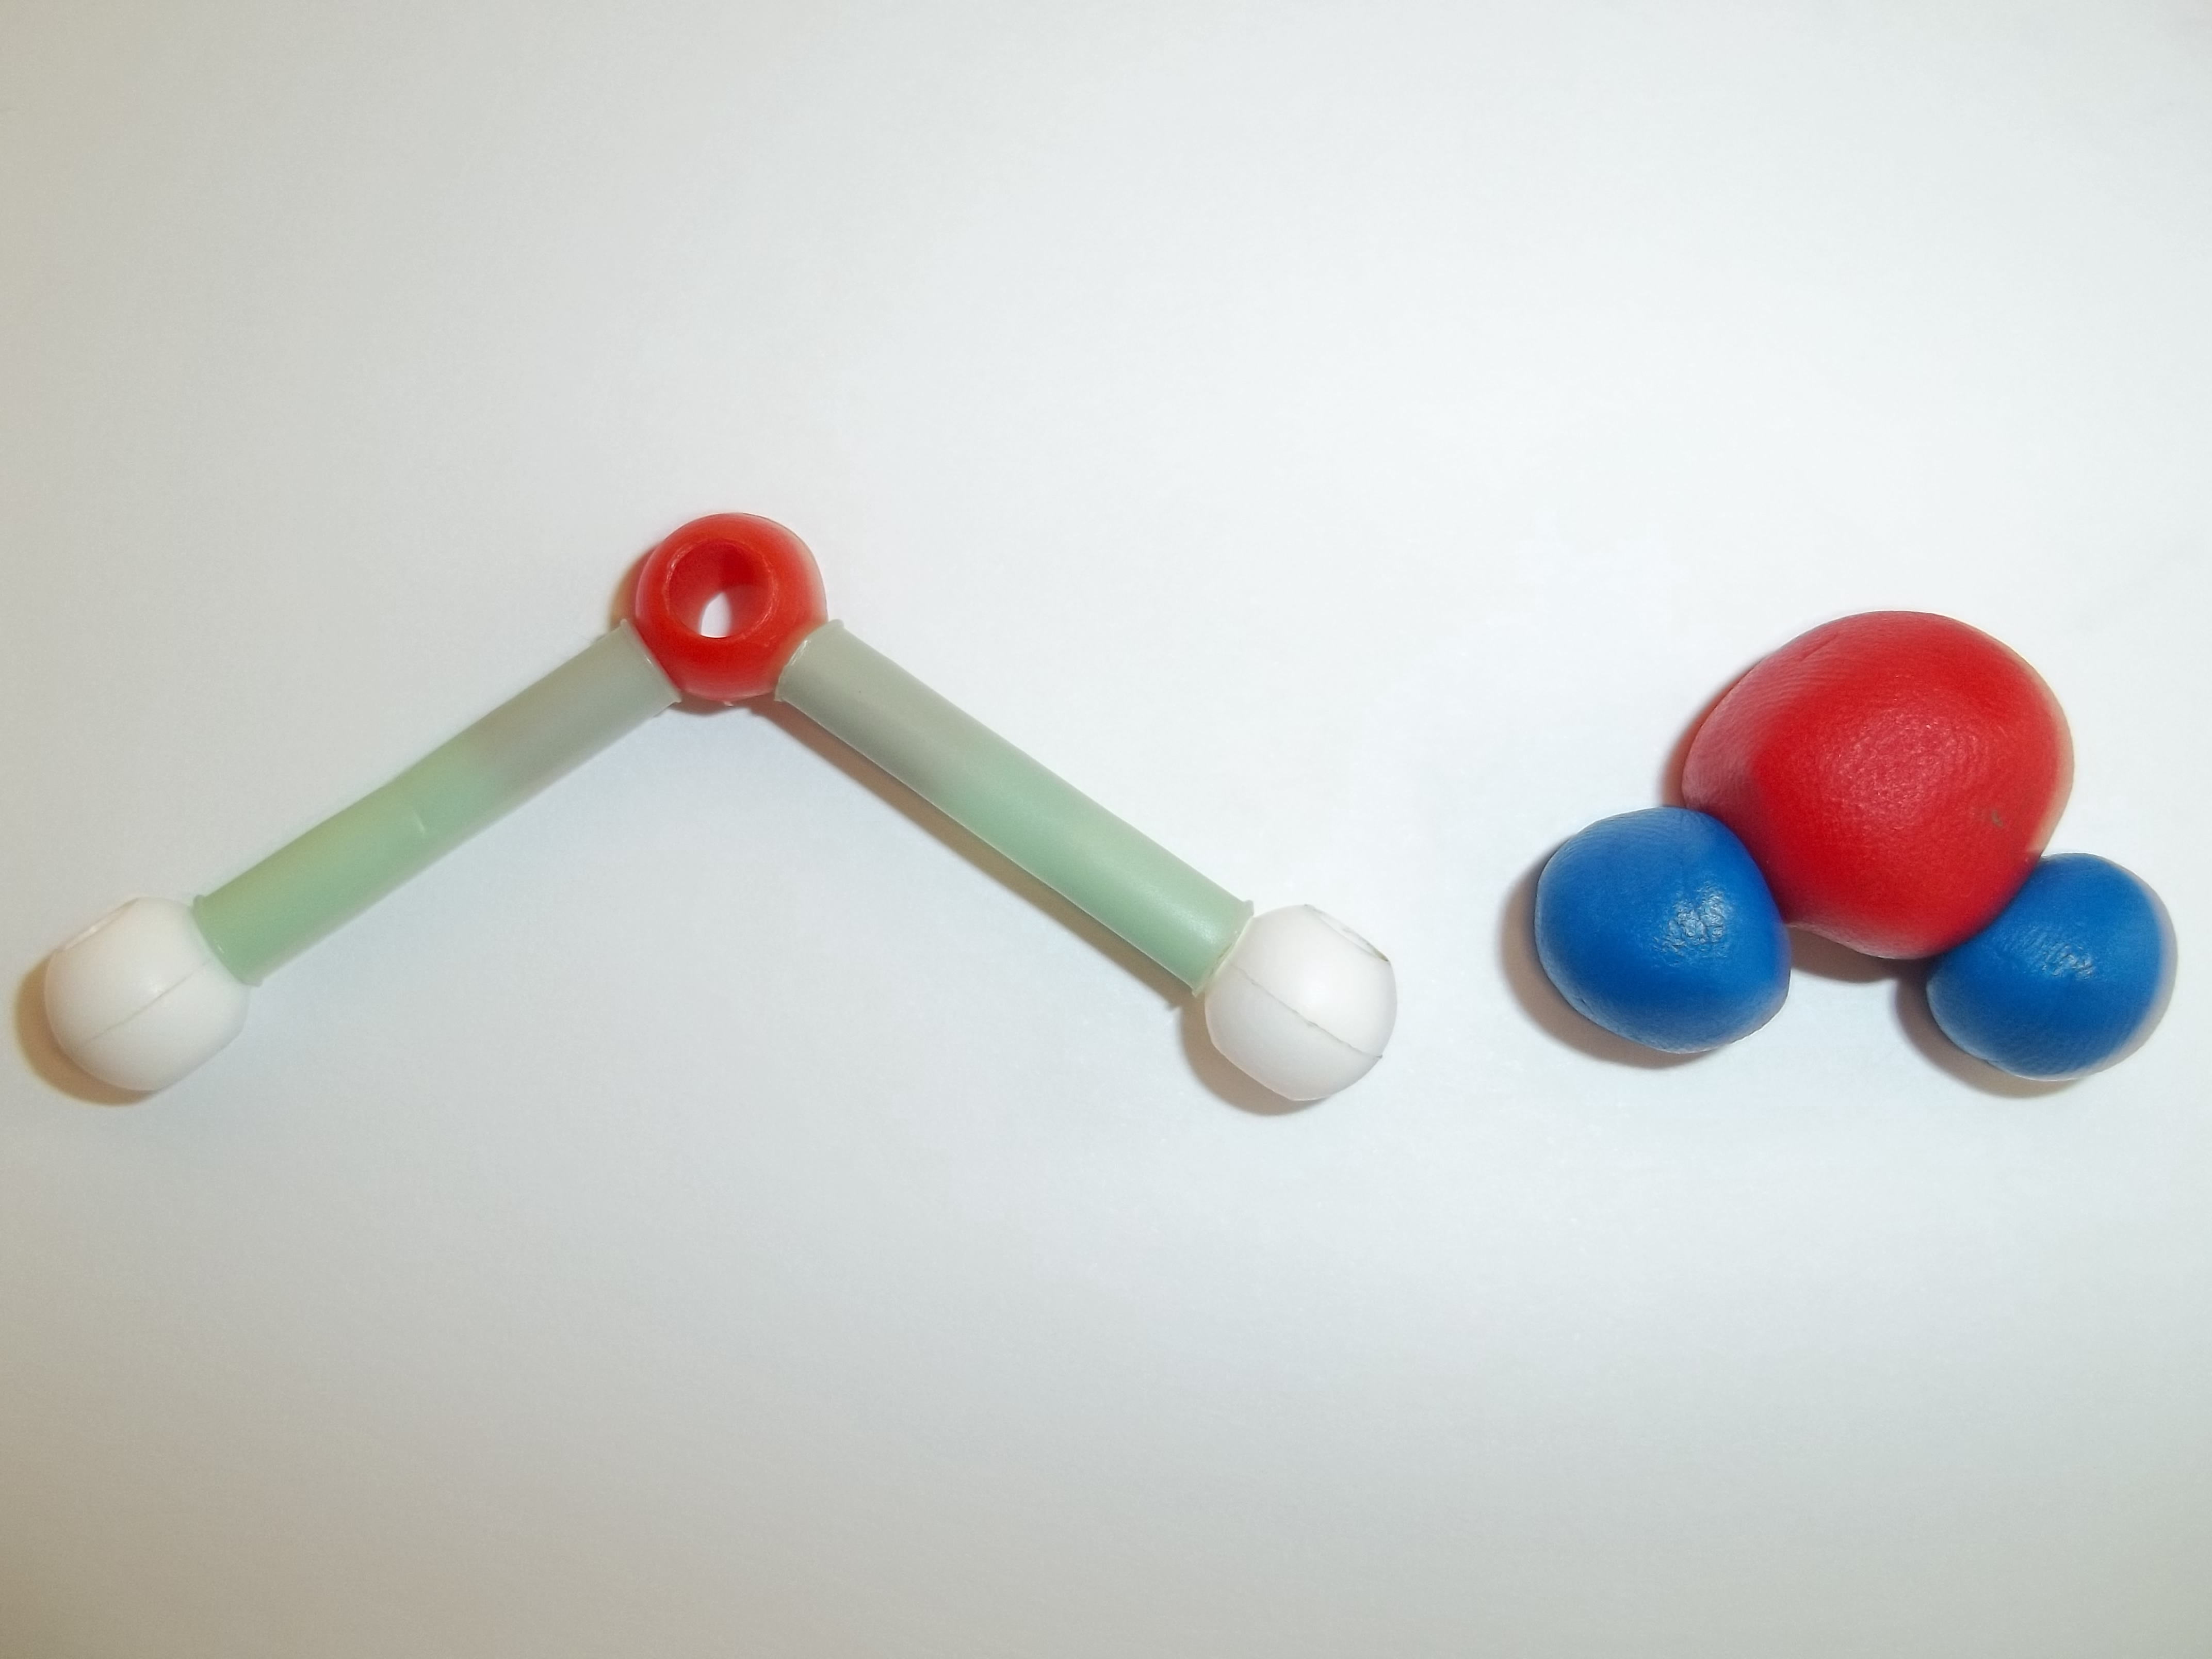
\includegraphics[width=0.4\textwidth]{photos/water.jpg}
\end{center}  
\begin{center}
\includegraphics[width=0.4\textwidth]{photos/ammonia.jpg}
\end{center}
\end{minipage}
\end{activity}
\Note{http://alteredqualia.com/canvasmol/ is a website that allows you to view several compounds. You do not need to know these compounds, this is simply to allow you to see one way of representing compounds.}
\mindsetvid{Reactions of acids and carbonates}{VPcbj}
\begin{g_experiment}{Investigating elements and compounds}
 \textbf{Aim:} \\
To investigate three reactions to learn about elements and compounds. \\
\textbf{Apparatus:} \\
\begin{minipage}{.5\textwidth}
\begin{itemize}[noitemsep]
 \item Cal-C-Vita tablet
\item test tubes
\item Bunsen burner
\item rubber stopper
\item delivery tube
\item lime water (a saturated solution of $\text{Ca(OH)}_{2}$)
\item candle
\item matches
\item copper sulphate ($\text{CuSO}_{4}\cdot 5\textsf{H}_{2}\textsf{O}$)
\item zinc metal
\item hydrochloric acid ($\text{HCl}$)
\end{itemize}
\end{minipage}
\begin{minipage}{.5\textwidth}
\begin{center}
\scalebox{0.9} % Change this value to rescale the drawing.
{
\begin{pspicture}(0,-1.387)(2.556,1.402)
\pspolygon[linewidth=0.03,fillstyle=solid,fillcolor=black](0.04,0.34699997)(0.62,0.34699997)(0.62,0.807)(0.04,0.807)
\rput{180.0}(0.68,-2.106){\psarc[linewidth=0.04](0.34,-1.053){0.31400025}{0.0}{180.0}}
\psline[linewidth=0.04cm](0.02,-1.0730001)(0.02,0.627)
\psline[linewidth=0.04cm](0.656,-1.0730001)(0.656,0.627)
\rput{30.256437}(-0.5475818,-0.38053852){\psellipse[linewidth=0.04,dimen=outer,fillstyle=solid,fillcolor=black](0.43,-1.2030001)(0.21,0.07)}
\psline[linewidth=0.04cm](0.0,-0.953)(0.64,-0.953)
\pscircle[linewidth=0.02,dimen=outer](0.31,-1.143){0.03}
\pscircle[linewidth=0.02,dimen=outer](0.41,-1.103){0.03}
\pscircle[linewidth=0.02,dimen=outer](0.25,-1.243){0.03}
\pscircle[linewidth=0.02,dimen=outer](0.27,-1.043){0.03}
\pscircle[linewidth=0.02,dimen=outer](0.47,-1.0630001){0.03}
\pscircle[linewidth=0.02,dimen=outer](0.39,-1.023){0.03}
\rput{180.0}(4.44,-2.106){\psarc[linewidth=0.04](2.22,-1.053){0.31400025}{0.0}{180.0}}
\psline[linewidth=0.04cm](1.9,-1.0730001)(1.9,0.627)
\psline[linewidth=0.04cm](2.536,-1.0730001)(2.536,0.627)
\psline[linewidth=0.03cm,doubleline=true,doublesep=0.06](0.36,0.12699997)(0.36,1.287)
\psline[linewidth=0.03cm,doubleline=true,doublesep=0.06](0.4,1.327)(2.18,1.327)
\psline[linewidth=0.03cm,doubleline=true,doublesep=0.06](2.24,1.3069999)(2.24,0.0069999695)
\psline[linewidth=0.03cm](0.4,1.367)(0.31,1.367)
\psline[linewidth=0.03cm](0.31,1.287)(0.31,1.367)
\psline[linewidth=0.03cm](2.274,1.367)(2.156,1.367)
\psline[linewidth=0.03cm](2.28,1.3069999)(2.28,1.387)
\psline[linewidth=0.03cm](1.9,0.30699998)(2.18,0.30699998)
\psline[linewidth=0.03cm](2.28,0.30699998)(2.52,0.30699998)
\pscircle[linewidth=0.02,dimen=outer](2.18,-0.03300003){0.02}
\pscircle[linewidth=0.02,dimen=outer](2.28,-0.07300003){0.02}
\pscircle[linewidth=0.02,dimen=outer](2.22,-0.13300003){0.02}
\end{pspicture} 
}
\scalebox{0.6}{
\begin{pspicture}(0,0)(5,5)
\newpsstyle{white} {linestyle=solid,linewidth=.1,fillstyle=solid,fillcolor=white}
\pstTubeEssais[niveauLiquide1=30,aspectLiquide1=white,solide={\pstGrenailleZinc[50]}]
\end{pspicture}
}
\scalebox{0.5}{
\begin{pspicture}(0,0)(5,5)
\newpsstyle{blue} {fillstyle=solid,fillcolor=white}
\pstChauffageTube[niveauLiquide1=20,aspectLiquide1=blue,solide={\pstClouFer[100]}]
\end{pspicture}
}
\end{center}
\end{minipage}
\textbf{Method:} \\
\textsl{Reaction 1}
\begin{enumerate}[label=\textbf{\arabic*}.]
\item Pour clear lime water into a test tube.
\item Into a second test tube place a Cal-C-Vita tablet. Cover the tablet with water and immediately place a stopper and delivery tube into the test tube.
\item Place the other end of the delivery tube into the lime water in the first test tube. Allow it to bubble for 1-2 minutes.
\item Now remove the stopper from the second test tube and hold a lit candle at the mouth of the test tube.
\item Record your observations.
\end{enumerate}
\textsl{Reaction 2}
\begin{enumerate}[label=\textbf{\arabic*}.]
\item Place a few drops of zinc metal in a test tube and cover the pieces with dilute hydrochloric acid.
\item Record your observations.
\item Now hold a burning match in the mouth of the test tube and observe what happens.
\end{enumerate}
\textsl{Reaction 3}
\begin{enumerate}[label=\textbf{\arabic*}.]
\item Place a spatula full of copper sulphate crystals into a test tube and heat the tube over a Bunsen burner.
\item Record your observations.
\end{enumerate}
\textbf{Discussion and conclusion:}\\
In the first reaction the lime water goes milky due to the presence of carbon dioxide. (Lime water can be used to detect carbon dioxide gas.) The carbon dioxide gas comes from the sodium bicarbonate ($\textsf{NaHCO}_3$) in the tablet. When you hold the candle over the test tube, the carbon dioxide snuffs out the candle flame. \\
In the second reaction bubbles of hydrogen gas form. Zinc reacts with the hydrochloric acid to form zinc chloride and hydrogen gas. \\
In the third reaction the copper sulphate crystals go white and droplets of water form on the sides of the test tube. The copper sulphate crystals have lost their water of crystallisation. 
\end{g_experiment}
% \pagebreak
\mindsetvid{Electrolysis of water}{VPbec}
\begin{g_experiment}{The electrolysis of water}
\textbf{Aim:} \\
To investigate the elements that make up water.\\
\textbf{Apparatus:}\\
\begin{minipage}{.4\textwidth}
\begin{itemize}[noitemsep]
 \item water
\item two pencils sharpened at both ends
\item 9 volt battery
\item connecting wire
\item tape
\item table salt or sodium sulphate
\end{itemize}
\end{minipage}
\begin{minipage}{.6\textwidth} 
\begin{center}
   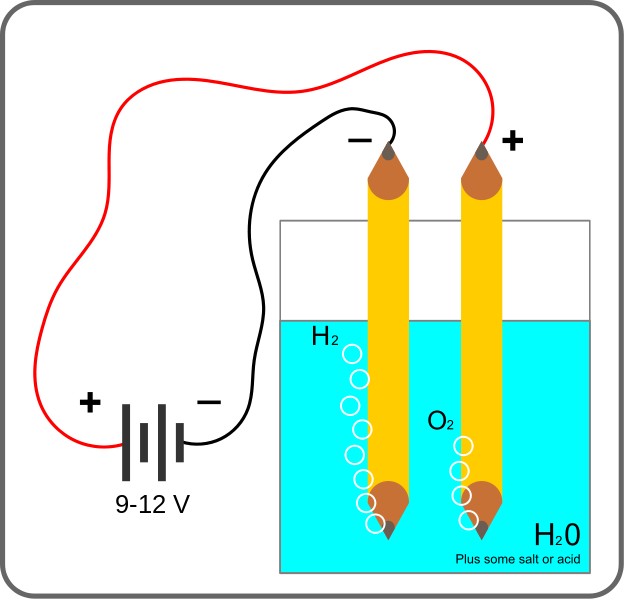
\includegraphics[width=0.5\textwidth]{photos/electrolysis.png}\\
\begin{caption}image by Nevit Dilmen\end{caption}
\end{center}
\end{minipage} \nopagebreak
\textbf{Method:}\\
Set up the apparatus as shown above. Observe what happens.\\
\textbf{Results:}\\
You should observe bubbles forming at the tips of the pencils. Oxygen gas is formed at the positive side and hydrogen at the negative side. 
\end{g_experiment}
\summary{xxx}
            \nopagebreak
%            \label{m38120*cid7} $ \hspace{-5pt}\begin{array}{cccccccccccc}   \end{array} $ \hspace{2 pt}\raisebox{-0.2em}{
\includegraphics[height=1em]{../icons/www.pdf}} {(section shortcode: P10055 )} \par 
\begin{itemize}[noitemsep]
\item The smallest unit of matter is the \textbf{atom}. Atoms can combine to form \textbf{compounds}.
\item A \textbf{compound} is a group of two or more different atoms that are attracted to each other by relatively strong forces or bonds. The atoms are combined in definite proportions.
\item In a compound, atoms are held together by \textbf{chemical bonds}. Covalent bonds, ionic bonds and metallic bonds are examples of chemical bonds.
\item A \textbf{covalent bond} exists between non-metal atoms. An \textbf{ionic bond} exists between non-metal and metal atoms and a \textbf{metallic bond} exists between metal atoms.
\item \textbf{Covalent molecular structures} interact and exist as separate molecules.
\item \textbf{Network structures} exist as giant repeating lattices. Network structures can consist of covalent, ionic or metallic compounds. 
\item A chemical formula is an abbreviated (shortened) way of describing a compound.
\item The \textbf{molecular formula} is a concise way of expressing information about the atoms that make up a particular covalent molecular compound. The molecular formula gives the exact number of each type of atom in the molecule.
\item The \textbf{empirical formula} is a way of expressing the relative number of each type of atom in a chemical compound. The empirical formula does not show the exact number of atoms, but rather the simplest ratio of the atoms in the compound.
\item The structure of a compound can be represented by stick, ball-and-stick or space-filling models.
\item A \textbf{stick} model use coloured sticks to represent compounds.
\item A \textbf{ball-and-stick} model is a 3-dimensional molecular model that uses 'balls' to represent atoms and 'sticks' to represent the bonds between them.
\item A \textbf{space-filling model} is also a 3-dimensional molecular model. The atoms are represented by spheres.
\end{itemize}
\label{m38120*secfhsst!!!underscore!!!id497}
            \begin{eocexercises}{Composition of matter}
            \nopagebreak \noindent
            \label{m38120*id311490}\begin{enumerate}[noitemsep, label=\textbf{\arabic*}. ] 
%Question 1
            \label{m38120*uid87}\item Give one word or term for each of the following 
descriptions.
\label{m38120*id34411506}\begin{enumerate}[noitemsep, label=\textbf{\alph*}. ] 
            \label{m38120*uid90}\item A composition of two or more atoms that act as a unit.
\label{m38120*uid9221}\item Chemical formula that gives the relative number of atoms 
of each element that are in a molecule.
\end{enumerate}
%Question 2
\label{m38120*uid227}\item Give a definition for each of the following terms: 
\label{m38120*id311506}\begin{enumerate}[noitemsep, label=\textbf{\alph*}. ] 
            \label{m38120*uid930}\item molecule
\label{m38120*uid91}\item ionic compound
\item covalent network structure
\item empirical formula
\item ball-and-stick model\end{enumerate}
%Question 3
\label{m38120*uid92}\item Ammonia, an ingredient in household cleaners, is made up of one part nitrogen ($\text{N}$) and three parts hydrogen ($\text{H}$). Answer the following questions:
\label{m38120*id311590}\begin{enumerate}[noitemsep, label=\textbf{\alph*}. ] 
            \label{m38120*uid94}\item is ammonia a covalent, ionic or metallic substance?
\label{m38120*uid95}\item write down the molecular formula for ammonia
\label{m38120*uid96}\item draw a ball-and-stick diagram
\label{m38120*uid97}\item draw a space-filling diagram
\end{enumerate}
%Question 4
            \label{m38120*uid11}\item In each of the following, say whether the chemical substance is made up of covalent, molecular structures, covalent network structures, ionic network structures or metallic structures:
\label{m38120*id308055}\begin{enumerate}[noitemsep, label=\textbf{\alph*}. ] 
            \label{m38120*uid12}\item ammonia gas (${\text{NH}}_{3}$)
\label{m38120*uid13}\item zinc metal ($\text{Zn}$)
\label{m38120*uid14}\item graphite ($\text{C}$)
\label{m38120*uid15}\item nitric acid (${\text{HNO}}_{3}$)
\label{m38120*uid16}\item potassium bromide ($\text{KBr}$)
\end{enumerate}
%Questin 5
\label{m38120*uid17}\item Refer to the diagram below and then answer the 
questions that follow:
    \setcounter{subfigure}{0}
	\begin{figure}[H] % horizontal\label{m38120*id308155}
\begin{center}
\scalebox{0.8}{
\begin{pspicture}(-2.6,-2.4)(6,2)
\SpecialCoor
%\psgrid[gridcolor=lightgray]

\psset{unit=0.5}

\pscircle[fillcolor=red,fillstyle=solid](2,0){1.5}
\pscircle[fillcolor=blue,fillstyle=solid](0,0){2}
\pscircle[fillcolor=red,fillstyle=solid](-2,0){1.5}
% \rput(-2,0){\pscurve(1.5;45)(-1.5;180)(1.5;-45)}

\psset{unit=1.5}
\rput(4,0){\pnode(-1,0){RO}\pnode(0,0){C}\pnode(1,0){LO}
\pnode(-1,0.075){ROO}\pnode(0,0.075){CO}\pnode(1,0.075){LOO}
\psline(RO)(C)
\psline(LO)(C)
\psline(ROO)(CO)
\psline(LOO)(CO)
\rput*(C){C}
\rput*(LO){O}
\rput*(RO){O}}
\end{pspicture}
}
\end{center}
 \end{figure}       \label{m38120*id308161}\begin{enumerate}[noitemsep, label=\textbf{\alph*}. ] 
            \label{m38120*uid18}\item Identify 
the molecule.
\label{m38120*uid19}\item Write the molecular formula for the molecule.
\label{m38120*uid20}\item Is the molecule a covalent, ionic or metallic substance? Explain.
\end{enumerate}
%Question 6
\label{m38120*uid21}\item Represent each of the following molecules using its 
\textsl{chemical formula}, \textsl{structural formula} and the \textsl{ball-and-stick model}.
\label{m38120*id308228}\begin{enumerate}[noitemsep, label=\textbf{\alph*}. ] 
            \item nitrogen\item carbon dioxide\item methane\item argon\end{enumerate}
\end{enumerate}
  \label{m38120**end}
\practiceinfo
\par 
 \par \begin{tabular}[h]{cccccc}
 (1.) l2e  &  (2.) l2M  &  (3.) ljQ  &  (4.) ljU  &   (5.) ljP  &  (6.) l2L    \end{tabular}
\end{eocexercises}
